% Example thesis body. All of the mainmatter chapters.
% Of course you can also input other TeX files as well.

\chapter{Example thesis body}

  \section{Figures}

    LaTeX's neat, but it can be frustrating sometimes. Here is an example figure to help keep you from running into reference / spacing issues. Order matters!

    \begin{figure}
      \centering%
      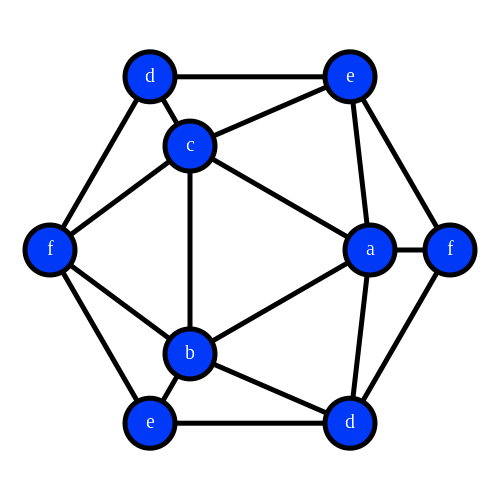
\includegraphics[scale=0.35]{res/images/pretty_picture.png}%
      \caption{A beautiful depiction of something.}%
      \label{fig:pretty_picture}
    \end{figure}

    See Figure~\ref{fig:pretty_picture} for a pretty picture. Isn't it lovely? By the way, it is much easier to include PNGs than SVGs in LaTeX. 

    \lipsum{17}

  \section{Tables}

    LaTeX's neat, but it can be frustrating sometimes. See Table~\ref{table:cool_table} for an example table to help keep you from running into reference / spacing issues. University requirements say that the caption should be above the table, which is why it is the way it is.

      \begin{table}
        \centering%
        \caption{What a cool table}%
        \label{table:cool_table}%
        \tablecaptionpadding{}%
        \begin{tabular}{c|cc}
          \diagbox{\(a\)}{\(b\)} & 0 & 1 \\\midrule
          0 & 0 & 0 \\
          1 & 1 & 0 \\
        \end{tabular}
      \end{table}


    \lipsum{17}
  
  \section{References}

    I like to do my references this way, but it is not a hard requirement. I used the \code{natbib} package to create granular author / year citations with \code{hyperref} support.

    Examples:
    \begin{itemize}
      \item Author and year:~\cite{vella:cat_breeding}
      \item Author only:~\citeauthoronly{vella:cat_breeding}
      \item Year only:~\citeyearonly{vella:cat_breeding}
    \end{itemize}

\blinddocument{}